\documentclass[12pt]{article}

\usepackage{pablo}
\usepackage{calc}
\usepackage[paperwidth=21cm,paperheight={29.7cm/4},margin=.5cm]{geometry}
\pagestyle{empty}

\begin{document}

\begin{center}
  \begin{tabular}{cc}

    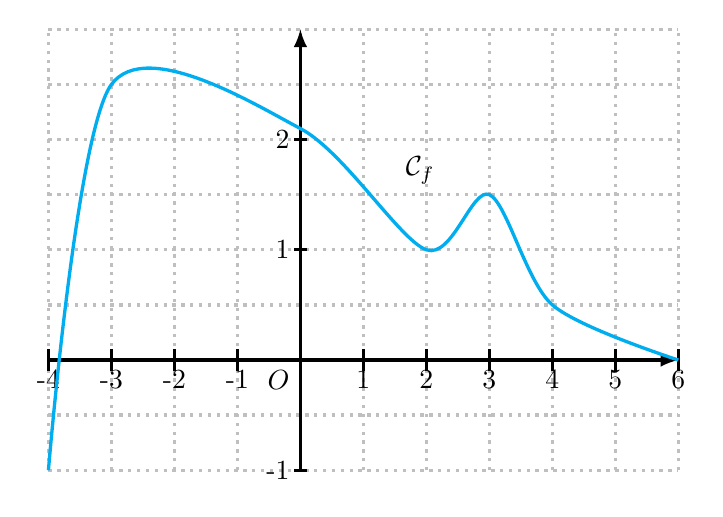
\begin{tikzpicture}[very thick,xscale=.8, yscale=1.4]
      \draw[dotted, lightgray, xstep=1, ystep=.5] (-4, -1) grid (6, 3);
      \draw[-latex] (-4,0) -- (6,0);
      \draw[-latex] (0,-1) -- (0,3);
      \foreach \x in {-4, -3, -2, -1, 1, 2, 3, 4, 5, 6} {
        \draw (\x,0) node[below]{\x};
        \draw (\x,{0.1}) -- (\x,{-0.1});
      }
      \foreach \y in {-1, 1, 2} {
        \draw (0,\y) node[left]{\y};
        \draw (-.1, \y) -- (.1, \y);
      }
      \draw [cyan] plot [smooth, tension=0.5] coordinates {
        (-4,-1)
        (-3, 2.5)
        (0, 2.1)
        (2, 1)
        (3, 1.5)
        (4, .5)
        (6, 0)
      };
      \draw (0,0) node[below left]{$O$};
      \draw (1.5, 1.5) node[above right]{$\mathcal{C}_f$};
    \end{tikzpicture}

    &

    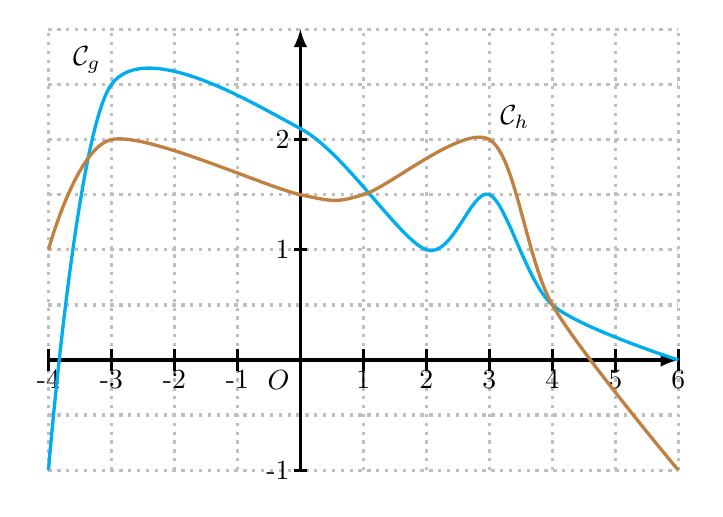
\begin{tikzpicture}[very thick,xscale=.8, yscale=1.4]
      \draw[dotted, lightgray, xstep=1, ystep=.5] (-4, -1) grid (6, 3);
      \draw[-latex] (-4,0) -- (6,0);
      \draw[-latex] (0,-1) -- (0,3);
      \foreach \x in {-4, -3, -2, -1, 1, 2, 3, 4, 5, 6} {
        \draw (\x,0) node[below]{\x};
        \draw (\x,{0.1}) -- (\x,{-0.1});
      }
      \foreach \y in {-1, 1, 2} {
        \draw (0,\y) node[left]{\y};
        \draw (-.1, \y) -- (.1, \y);
      }
      \draw [cyan] plot [smooth, tension=0.5] coordinates {
        (-4,-1)
        (-3, 2.5)
        (0, 2.1)
        (2, 1)
        (3, 1.5)
        (4, .5)
        (6, 0)
      };
      \draw [brown] plot [smooth, tension=0.5] coordinates {
        (-4,1)
        (-3, 2)
        (0, 1.5)
        (1, 1.5)
        (3, 2)
        (4, .5)
        (6, -1)
      };
      \draw (0,0) node[below left]{$O$};
      \draw (-3, 2.5) node[above left]{$\mathcal{C}_g$};
      \draw (3, 2) node[above right]{$\mathcal{C}_h$};
    \end{tikzpicture}

  \end{tabular}
\end{center}

\end{document}
